% !TeX root = ../regression_logistique.tex
\chapter{Géométrie en dimension quelconque}
\label{ann:geometrie}

\orient{%
écrire l'équation d'une frontière pour $n$ variables et en donner la dimension ;
décrire la région attribuée à une classe par la règle du maximum et énoncer ses
propriétés exactes}{%
produit scalaire et norme (\annexeref{ann:prerequis}) ; chapitres~\ref{ch:nuage}
et~\ref{ch:classifieur}}{%
approfondissement ; se saute sans rompre la lecture du fil principal}

\section{Frontière pour un nombre quelconque de matières}

Avec $n$ notes, une observation est un point de $\R^n$ et l'équation de la
frontière devient
\[
  w_0+w_1x_1+\dots+w_nx_n=0,
\]
soit une équation linéaire à $n$ inconnues, non triviale dès que
$(w_1,\dots,w_n)\neq0$. Son ensemble de solutions est un sous-espace affine de
dimension $n-1$ : une contrainte non dégénérée retire un degré de liberté. Cet
objet porte le nom d'\emph{hyperplan affine} de $\R^n$ --- droite pour $n=2$,
plan pour $n=3$, sans représentation graphique au-delà.

\begin{table}[htbp]
\centering
\begin{tabular}{ccccc}
\toprule
matières & espace des observations & frontière & sa dimension & coefficients \\
\midrule
$1$  & $\R$      & un point    & $0$ & $2$  \\
$2$  & $\R^2$    & une droite  & $1$ & $3$  \\
$3$  & $\R^3$    & un plan     & $2$ & $4$  \\
$n$  & $\R^n$    & un hyperplan & $n-1$ & $n+1$ \\
\midrule
$10$ & $\R^{10}$ & un hyperplan & $9$ & $11$ \\
\bottomrule
\end{tabular}
\caption{La frontière occupe une dimension de moins que l'espace des
observations et le sépare en deux demi-espaces. Le nombre de coefficients croît
d'une unité par matière ajoutée.}
\label{tab:dimensions}
\end{table}

\begin{figure}[htbp]
\centering
\begin{graphique}{Trois vignettes. Pour une matière, un axe portant un point qui sépare disques et croix. Pour deux matières, un rectangle traversé par une droite. Pour trois matières, un repère en perspective traversé par un plan. Les dimensions 0, 1 et 2 sont indiquées sous chacune.}
\begin{tikzpicture}[baseline=(current bounding box.north),font=\footnotesize,
  alt={En dimension un, un point sur un axe sépare les observations des deux classes.}]
\node[font=\small,anchor=south] at (1.6,1.5) {$n=1$};
\draw[ink!45] (0,0.4) -- (3.2,0.4);
\foreach \x in {0.3,0.6,0.95,1.25}{\fill[accent] (\x,0.4) circle (1.5pt);}
\foreach \x in {1.95,2.25,2.6,2.95}{
  \draw[warning!80,line width=.7pt] (\x-.06,0.34) -- (\x+.06,0.46);
  \draw[warning!80,line width=.7pt] (\x-.06,0.46) -- (\x+.06,0.34);}
\fill[ink] (1.6,0.4) circle (2.2pt);
\node[anchor=north,text=ink] at (1.6,0.25) {un point};
\node[anchor=north,text=ink!70,font=\scriptsize] at (1.6,-0.15)
  {dimension $0$};
\end{tikzpicture}\hfill
\begin{tikzpicture}[baseline=(current bounding box.north),font=\footnotesize,
  alt={En dimension deux, une droite dans un plan sépare les observations des deux classes.}]
\node[font=\small,anchor=south] at (1.6,1.5) {$n=2$};
\draw[gridgray!60] (0,-0.35) rectangle (3.2,1.35);
\draw[ink,very thick] (0.25,-0.1) -- (2.95,1.1);
\foreach \p in {(0.6,0.9),(1.0,1.15),(1.5,1.25)}{\fill[accent] \p circle (1.5pt);}
\foreach \p/\qx/\qy in {(1.5,0.1)/1.5/0.1,(2.2,0.35)/2.2/0.35,(2.6,0.15)/2.6/0.15}{
  \draw[warning!80,line width=.7pt] (\qx-.06,\qy-.06) -- (\qx+.06,\qy+.06);
  \draw[warning!80,line width=.7pt] (\qx-.06,\qy+.06) -- (\qx+.06,\qy-.06);}
\node[anchor=north,text=ink] at (1.6,-0.45) {une droite};
\node[anchor=north,text=ink!70,font=\scriptsize] at (1.6,-0.85)
  {dimension $1$};
\end{tikzpicture}\hfill
\begin{tikzpicture}[baseline=(current bounding box.north),font=\footnotesize,
  alt={En dimension trois, un plan dans l'espace sépare les observations des deux classes.}]
\node[font=\small,anchor=south] at (1.6,1.5) {$n=3$};
\draw[ink!45,-{Latex[length=1.6mm]}] (0.9,0.3) -- (2.9,0.3);
\draw[ink!45,-{Latex[length=1.6mm]}] (0.9,0.3) -- (1.6,0.85);
\draw[ink!45,-{Latex[length=1.6mm]}] (0.9,0.3) -- (0.9,1.4);
\fill[ink!22,draw=ink!60] (0.35,0.45) -- (2.35,-0.15) -- (2.95,0.55)
  -- (0.95,1.15) -- cycle;
\foreach \p in {(1.1,0.95),(1.7,0.8)}{\fill[accent] \p circle (1.5pt);}
\foreach \qx/\qy in {1.6/0.15,2.3/0.35}{
  \draw[warning!80,line width=.7pt] (\qx-.06,\qy-.06) -- (\qx+.06,\qy+.06);
  \draw[warning!80,line width=.7pt] (\qx-.06,\qy+.06) -- (\qx+.06,\qy-.06);}
\node[anchor=north,text=ink] at (1.6,-0.45) {un plan};
\node[anchor=north,text=ink!70,font=\scriptsize] at (1.6,-0.85)
  {dimension $2$};
\end{tikzpicture}
\end{graphique}
\caption{Frontière pour une, deux et trois matières. Disque : classe traitée ;
croix : autres classes. Le vecteur normal, $|z|/\|w\|$ et le signe de $z$
conservent leur rôle.}
\label{fig:dimensions}
\end{figure}
\FloatBarrier

Les formules du fil principal s'écrivent avec un nombre quelconque de notes, et
les démonstrations des annexes suivantes valent pour $n$ quelconque. Deux
matières servent en partie~I parce qu'elles se dessinent ; le modèle complet du
projet en retient dix.

\section{Rôle de chaque coefficient}

Les trois coefficients agissent séparément : $(w_1,w_2)$ fixe la direction de la
frontière et $w_0$ sa position. La norme $\|w\|$ laisse la frontière en place et
fixe la vitesse à laquelle $z$ croît lorsqu'on s'en éloigne
(ch.~\ref{ch:descente}).

\begin{figure}[htbp]
\centering
\begin{graphique}{Un plan quadrillé traversé par une droite oblique séparant deux demi-plans teintés, marqués z positif et z négatif. Depuis le pied de la perpendiculaire issue de l'origine part un vecteur normal ; un segment nommé d indice O joint l'origine à ce pied.}
\begin{tikzpicture}
\begin{axis}[width=.66\textwidth,axis equal image,
  axis lines=box,axis line style={ink!40},
  grid=major,grid style={gridgray!25},
  tick label style={font=\small},label style={font=\small},
  xlabel={$x_1$},ylabel={$x_2$},
  xmin=-2.2,xmax=2.2,ymin=-1.4,ymax=2.2,
  xtick={-2,-1,0,1,2},ytick={-1,0,1,2},
  domain=-2.2:2.2,samples=2,clip=true]

  \fill[accent!12] (axis cs:-2.2,-0.92) -- (axis cs:2.2,1.72)
    -- (axis cs:2.2,2.2) -- (axis cs:-2.2,2.2) -- cycle;
  \fill[warning!10] (axis cs:-2.2,-0.92) -- (axis cs:2.2,1.72)
    -- (axis cs:2.2,-1.4) -- (axis cs:-2.2,-1.4) -- cycle;

  \addplot[ink,very thick]{0.4+0.6*x};

  % angle droit entre la frontiere et sa normale, au pied H
  \addplot[ink!70,thin] coordinates
    {(-0.022,0.387) (-0.115,0.541) (-0.269,0.448)};

  \addplot[warning,-{Latex[length=2.6mm]},very thick]
    coordinates {(-0.176,0.294) (-0.776,1.294)};
  \addplot[accent,very thick] coordinates {(0,0) (-0.176,0.294)};
  \addplot[only marks,mark=*,ink,mark size=2pt]
    coordinates {(0,0) (-0.176,0.294)};

  \node[font=\small,text=accent,anchor=east] at (axis cs:-0.20,0.16) {$d_O$};

  \node[font=\small,text=warning,anchor=south] at (axis cs:-0.776,1.36)
    {$(w_1,w_2)$};
  \node[font=\scriptsize,text=ink,anchor=north east] at (axis cs:-0.05,-0.04)
    {$O$};
  \node[font=\small,text=ink,fill=white,inner sep=1.5pt,anchor=south east]
    at (axis cs:2.12,1.70) {$z=0$};
  \node[font=\small,text=accent!80!black,anchor=north west]
    at (axis cs:-2.08,2.12) {$z>0$};
  \node[font=\small,text=warning,anchor=south east]
    at (axis cs:2.08,-1.32) {$z<0$};
\end{axis}
\end{tikzpicture}
\end{graphique}
\caption{Frontière $-0{,}4-0{,}6x_1+x_2=0$ et son vecteur normal
$(-0{,}6\,;1)$, tracé à l'échelle depuis le pied de la perpendiculaire issue de
l'origine. Le segment $d_O$ mesure $-w_0/\|w\|=0{,}343$.}
\label{fig:normal}
\end{figure}
\FloatBarrier

Les deux panneaux suivants font varier un coefficient à la fois à partir de
$w=(0\,;0{,}8\,;1)$. Ils couvrent tous les cas : la frontière ne dépend que de la
direction de $(w_1,w_2)$, et faire varier $w_1$ à $w_2$ fixé parcourt cette
direction tout entière.

\begin{figure}[htbp]
\centering
\begin{graphique}{Deux panneaux. À gauche, trois droites parallèles correspondant à trois valeurs du biais. À droite, trois droites concourantes à l'origine correspondant à trois valeurs du premier coefficient. Le trait plein est commun aux deux panneaux.}
\begin{tikzpicture}[baseline=(current bounding box.north),
  alt={Trois frontières parallèles obtenues en faisant varier le biais, les deux autres coefficients restant fixes.}]
\begin{axis}[panel,width=.40\textwidth,height=5.6cm,
  title={variation de $w_0$\\[-1pt] \scriptsize $w_1=0{,}8$,\ $w_2=1$},
  title style={align=center},xlabel={$x_1$},ylabel={$x_2$},
  legend style={at={(0.5,-0.32)},anchor=north,draw=none,font=\scriptsize,
    cells={anchor=west},row sep=-1.5pt,legend image post style={scale=.7}},
  domain=-3:3,samples=2]
  \addplot[ink!45,thick,densely dashed]{-0.8*x+1.6};
  \addlegendentry{$w_0=-1{,}6$}
  \addplot[accent,very thick]{-0.8*x};
  \addlegendentry{$w_0=0$}
  \addplot[warning,thick,densely dotted]{-0.8*x-1.6};
  \addlegendentry{$w_0=+1{,}6$}
\end{axis}
\end{tikzpicture}\hfill
\begin{tikzpicture}[baseline=(current bounding box.north),
  alt={Trois frontières concourantes à l'origine obtenues en faisant varier le premier coefficient, le biais restant nul.}]
\begin{axis}[panel,width=.40\textwidth,height=5.6cm,
  title={variation de $w_1$\\[-1pt] \scriptsize $w_0=0$,\ $w_2=1$},
  title style={align=center},xlabel={$x_1$},yticklabels={},
  legend style={at={(0.5,-0.32)},anchor=north,draw=none,font=\scriptsize,
    cells={anchor=west},row sep=-1.5pt,legend image post style={scale=.7}},
  domain=-3:3,samples=2]
  \addplot[ink!45,thick,densely dashed]{-0.2*x};
  \addlegendentry{$w_1=0{,}2$}
  \addplot[accent,very thick]{-0.8*x};
  \addlegendentry{$w_1=0{,}8$}
  \addplot[warning,thick,densely dotted]{-2.2*x};
  \addlegendentry{$w_1=2{,}2$}
\end{axis}
\end{tikzpicture}
\end{graphique}
\caption{Trait plein commun aux deux panneaux : $w=(0\,;0{,}8\,;1)$. À gauche,
$w_0$ translate la droite ; à droite, $w_1$ la fait pivoter autour de l'origine,
que $w_0=0$ laisse sur la frontière.}
\label{fig:trois-nombres}
\end{figure}
\FloatBarrier

\section{Forme des régions du classifieur}

La règle du score maximal (ch.~\ref{ch:classifieur}) attribue une classe à
chaque point du plan. Quelle forme prend l'ensemble des points attribués à une
classe donnée ?

Prenons \Gryf. Son modèle l'emporte en un point lorsque son score y dépasse les
trois autres, ce qui fait trois conditions. La première s'écrit
\[
  z_G\geq z_H
  \iff
  (w_{G0}-w_{H0})+(w_{G1}-w_{H1})x_1+(w_{G2}-w_{H2})x_2\geq 0 ,
\]
et les deux autres s'obtiennent en remplaçant $H$ par $R$ puis par $S$. Le membre
de gauche est une fonction affine des deux notes ; l'inégalité définit donc un
demi-plan, bordé par la droite où les deux scores s'égalisent.

\begin{figure}[htbp]
\centering
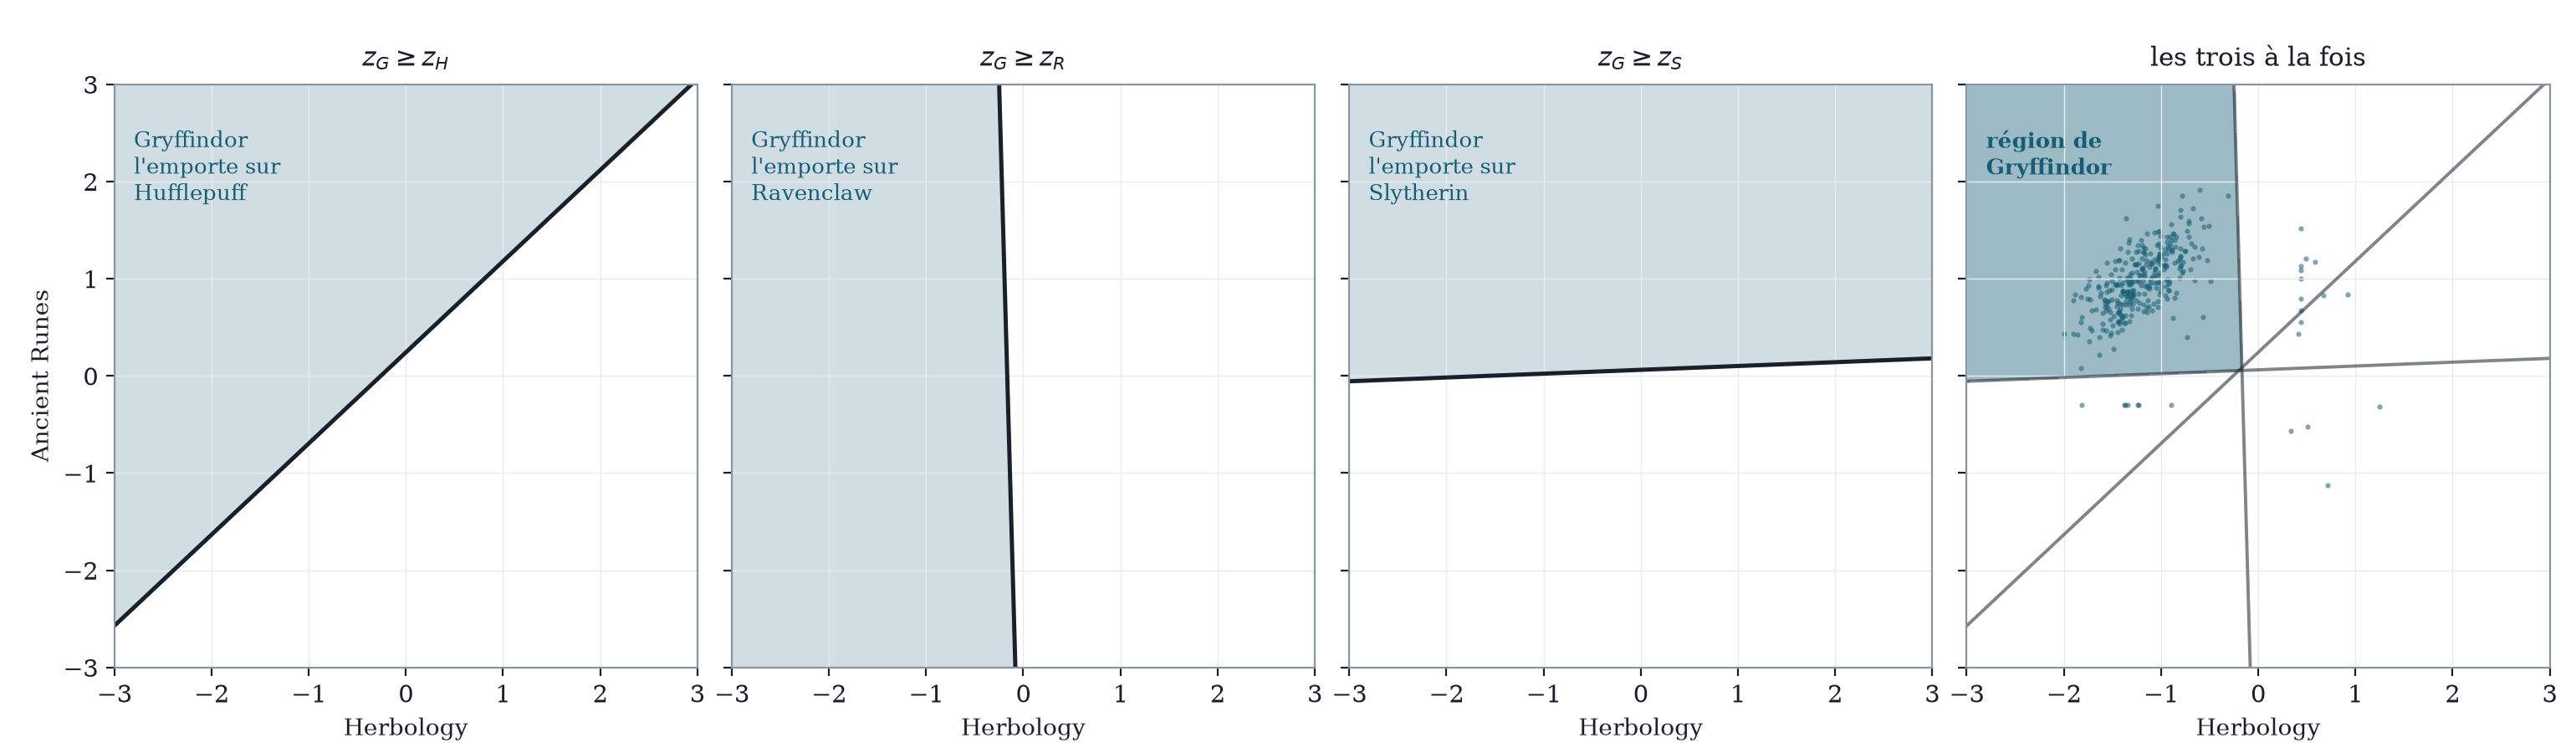
\includegraphics[width=\textwidth,
  alt={Quatre panneaux. Les trois premiers montrent chacun le demi-plan où le score de Gryffindor dépasse celui d'un rival. Le quatrième montre leur intersection, un polygone convexe non borné contenant presque toutes les observations de cette classe.}]{figures/demiplans.png}
\caption{Les trois demi-plans où \Gryf l'emporte sur chacun de ses rivaux, puis
leur intersection. Le dernier panneau porte les observations de cette classe,
qui s'y trouvent presque toutes. État du modèle : \Movr.}
\label{fig:demiplans}
\end{figure}
\FloatBarrier

La région de \Gryf est l'intersection de ces trois demi-plans : un ensemble
convexe, intersection finie de demi-plans, donc un polyèdre convexe du plan. Il
peut être vide, borné ou non borné. Trois propriétés en découlent, énoncées avec
leurs conditions.

\begin{enumerate}
  \item \textbf{Convexité.} Deux points d'une même région ont tout le segment
        qui les joint dans cette région. Une classe ne peut donc pas occuper
        deux zones séparées.
  \item \textbf{Bords.} Les bords sont portés par les droites d'égalité
        $z_G=z_j$, distinctes des quatre frontières binaires $z_k=0$. Un bord
        s'interrompt là où un troisième modèle prend le dessus. Si la région est
        bornée, ses arêtes sont de longueur finie ; si elle ne l'est pas ---
        ce qui arrive dès que la région contient une demi-droite --- au moins
        une arête est infinie. Sur les quatre modèles employés ici, les quatre
        régions sont non bornées.
  \item \textbf{Départage.} En cas d'égalité exacte entre deux scores maximaux,
        $\arg\max$ ne désigne pas une classe : il faut une convention. Le code
        de la partie~II retient le premier maximum rencontré dans l'ordre de la
        liste des classes. Cet événement est de probabilité nulle sur des
        données continues, mais se produit sur des valeurs arrondies.
\end{enumerate}

\begin{figure}[htbp]
\centering
\begin{graphique}{Un plan quadrillé traversé par trois droites : la frontière de Gryffindor en trait plein, celle de Ravenclaw en tireté, et en trait épais la limite entre leurs deux régions, presque verticale, portant son vecteur normal. Les trois se coupent en un même point.}
\begin{tikzpicture}[x=1.28cm,y=1.28cm,font=\footnotesize]
\begin{scope}
\clip (-3,-3) rectangle (3,3);
\fill[gryff!7]  (-3,-3) -- (-0.082,-3) -- (-0.248,3) -- (-3,3) -- cycle;
\fill[raven!7]  (-0.082,-3) -- (3,-3) -- (3,3) -- (-0.248,3) -- cycle;
\draw[gridgray!35] (-3,-3) grid[step=1] (3,3);
\draw[gryff,very thick] (-3,-1.611) -- (3,4.343);
\draw[raven,very thick,densely dashed] (-3,4.114) -- (3,-2.186);
\draw[ink,ultra thick] (-0.082,-3) -- (-0.248,3);
\draw[ink,-{Stealth[length=2.4mm]},thick]
  (-0.197,1.171) -- ++(-0.99,-0.028);
\end{scope}
\draw[ink!45] (-3,-3) rectangle (3,3);
\draw[ink!45] (-3,0) -- (3,0);   \draw[ink!45] (0,-3) -- (0,3);
\fill[white] (-0.197,1.171) circle (2.1pt);
\draw[ink,thick] (-0.197,1.171) circle (2.1pt);
\node[gryff,anchor=west,fill=white,inner sep=1pt] at (-2.95,-1.95) {$z_G=0$};
\node[raven,anchor=east,fill=white,inner sep=1pt] at (2.95,-1.95) {$z_R=0$};
\node[ink,anchor=south,fill=white,inner sep=1.5pt] at (-0.16,3.02)
  {$z_G=z_R$};
\node[ink,anchor=south east,font=\scriptsize] at (-1.20,1.22)
  {$w_G-w_R$};
\node[gryff!85,anchor=west] at (-2.9,2.3) {$z_G>z_R$};
\node[raven!85,anchor=east] at (2.9,2.3) {$z_R>z_G$};
\node[anchor=north] at (0,-3.15) {\Herb};
\node[anchor=south,rotate=90] at (-3.15,0) {\Runes};
\end{tikzpicture}
\end{graphique}
\caption{Frontières binaires de \Gryf (trait plein) et de \Rav (tireté), et limite entre
leurs deux régions (trait épais). Cette limite a pour vecteur normal $w_G-w_R$
et passe par l'intersection des deux premières.}
\label{fig:limite-paire}
\end{figure}
\FloatBarrier

Quatre classes forment six paires, donc six droites d'égalité, dont chacune ne
borde une région que sur la portion où le score commun aux deux classes dépasse
aussi les deux autres.

Cette construction se vérifie le long d'un trajet : chaque score y devient une
fonction affine du chemin parcouru, donc une droite, et le maximum des quatre
une ligne brisée dont les points anguleux marquent les changements de région.

\begin{figure}[htbp]
\centering
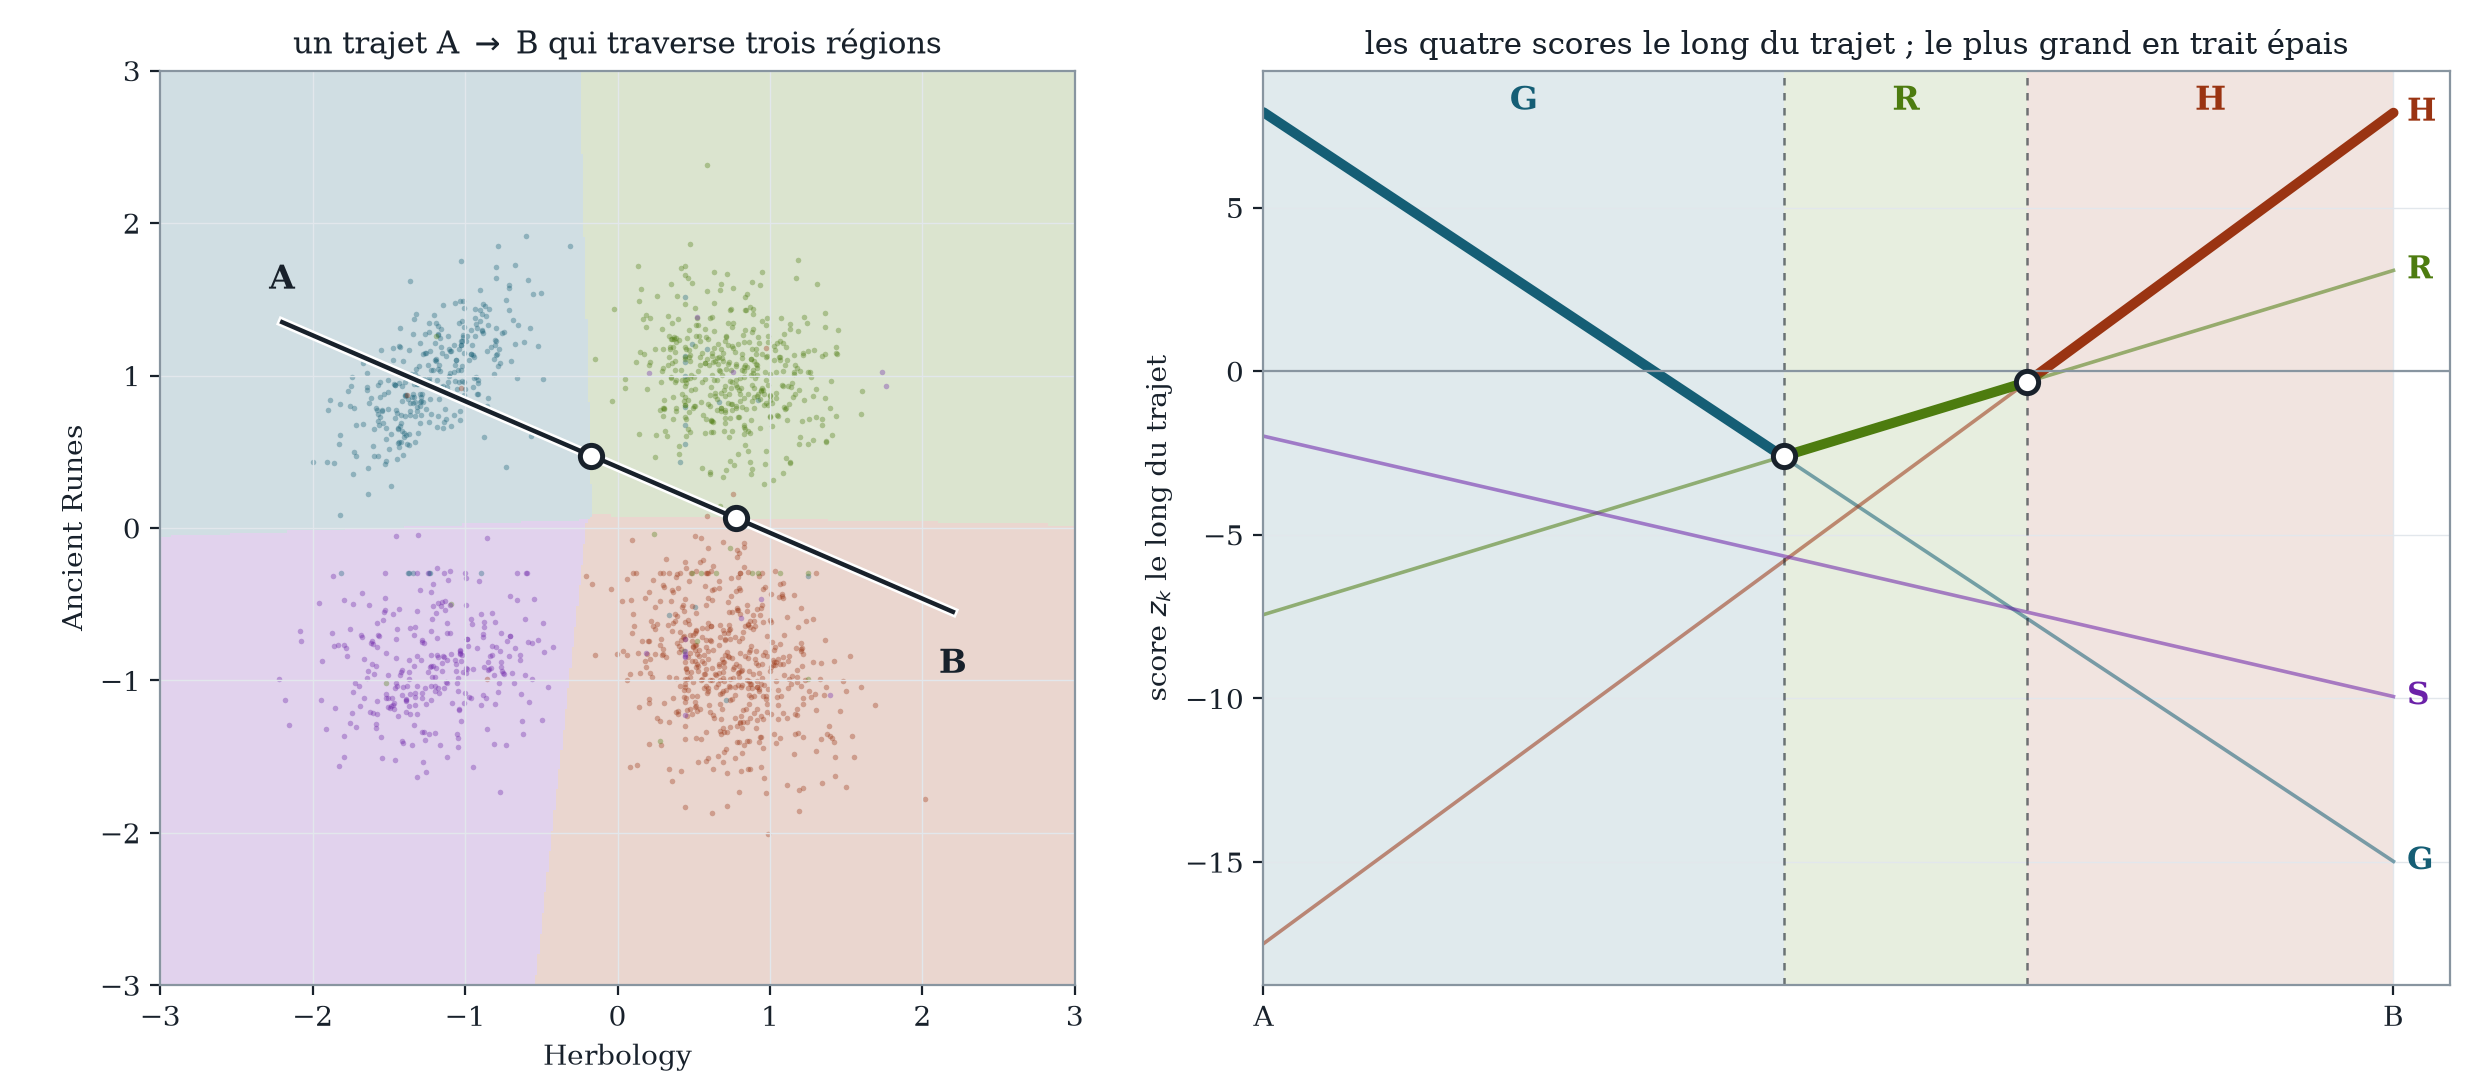
\includegraphics[width=\textwidth,
  alt={À gauche, un segment tracé dans le nuage du groupe des Gryffindor vers celui des Hufflepuff. À droite, les quatre scores relevés le long de ce segment, quatre droites ; leur maximum forme une ligne brisée à deux points anguleux marquant les changements de région.}]{figures/score_max.png}
\caption{Trajet de \Gryf vers \Huff, à gauche ; quatre scores et leur maximum, à
droite. Les angles de la ligne épaisse marquent les changements de région.}
\label{fig:score-max}
\end{figure}
\FloatBarrier
